\subsection{Objetivo 6 --- comparação com métodos reais}

\textit{Comparar a acurácia estimada pelos níveis de Oracle com classificadores
individuais e métodos reais de combinação (votação majoritária, média de
probabilidades) e, quando viável, DCS/DES.}

Foram medidos $14$ fusores nos $1450$ folds dos cinco modos, com DSEL disjunto e
$k=7$ vizinhos ($k=6$ nos pools de Perceptron, sem os dois métodos que exigem
\texttt{predict\_proba}). Esta seção detalha os três modos já publicados
(PGDCS-F1/T1, Bagging, Random Forest); o objetivo 4 (Seção~5) mostra que PGDCS
completo e bags aleatórios reproduzem o mesmo padrão do PGDCS-F1/T1 em todas as
métricas de pool, sem diferença estatística --- a tabela abaixo generaliza para os
três modos de Perceptron, não apenas o F1/T1.

\begin{table}[htbp]
\centering
\small
\caption{Acurácia média dos $14$ fusores contra o teto \On{1}. Traço $=$ método que
exige \texttt{predict\_proba}, indisponível no Perceptron linear.}
\begin{tabular}{lrrr}
\toprule
Fusor & PGDCS-F1/T1 & Bagging & Random Forest \\
\midrule
Votação majoritária (\mvr)      & 0.7784 & 0.8467 & 0.8549 \\
Combinação suave                & 0.7738 & 0.8466 & 0.8546 \\
\midrule
OLA                             & 0.7829 & 0.8028 & 0.7915 \\
LCA                             & 0.7271 & 0.7878 & 0.7863 \\
MCB                             & 0.7828 & 0.7943 & 0.7900 \\
Rank                            & 0.7760 & 0.8022 & 0.7908 \\
KNORA-E                         & 0.7897 & 0.8261 & 0.8274 \\
KNORA-U                         & \textbf{0.8056} & 0.8468 & \textbf{0.8564} \\
DES-P                           & 0.8021 & 0.8481 & 0.8566 \\
DES-KNN                         & 0.7995 & 0.8477 & 0.8492 \\
META-DES                        & ---    & \textbf{0.8482} & 0.8545 \\
KNOP                            & ---    & \textbf{0.8486} & 0.8556 \\
\midrule
Melhor individual (estático)    & 0.7630 & 0.7999 & 0.7958 \\
Seleção estática                & 0.7797 & 0.8475 & 0.8546 \\
\midrule
Melhor por fold (\emph{oracle} sobre métodos) & 0.8340 & 0.8688 & 0.8733 \\
Acurácia individual média       & 0.7052 & 0.7931 & 0.7806 \\
\On{1}                          & 0.9976 & 0.9951 & 0.9970 \\
\midrule
Folga $\On{1}-\mvr$             & 0.2192 & 0.1484 & 0.1421 \\
\textbf{Folga recuperada}       & \textbf{24.0\%} & \textbf{15.0\%} & \textbf{14.2\%} \\
\bottomrule
\end{tabular}
\end{table}

\begin{figure}[htbp]
\centering
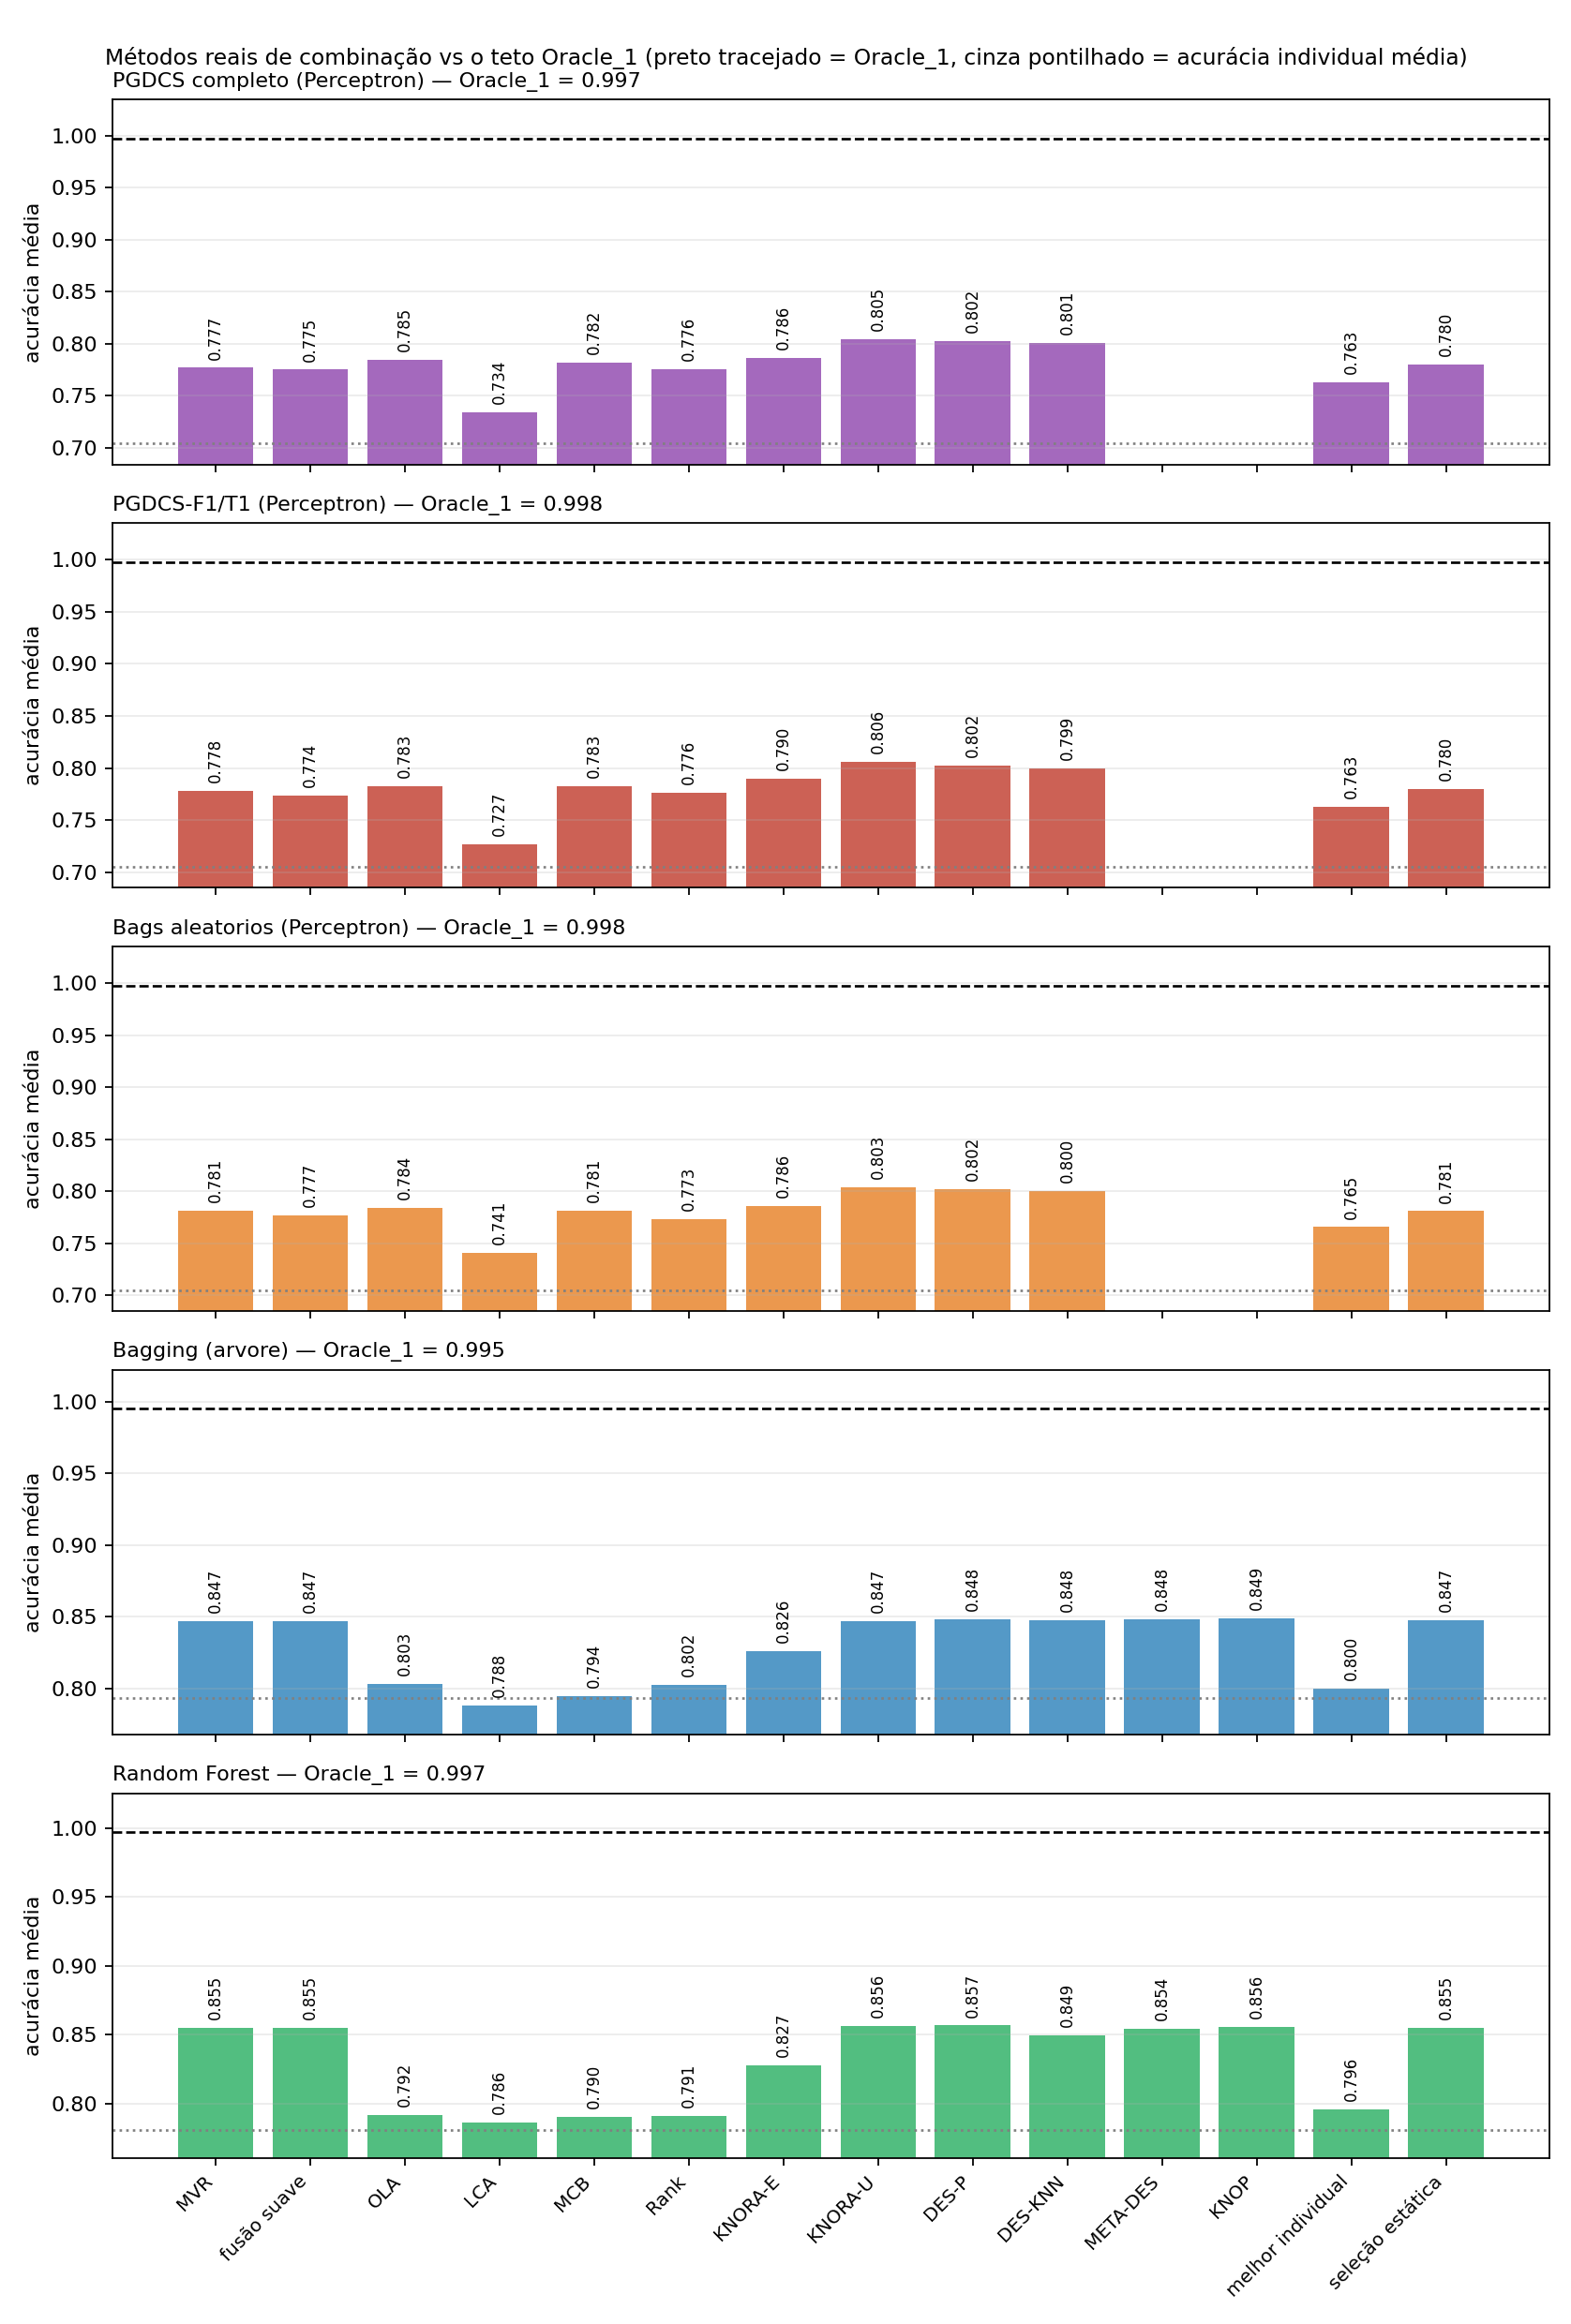
\includegraphics[width=0.95\textwidth]{figuras/fig7_fuser_accuracy.png}
\caption{Os $14$ fusores contra o teto \On{1} (tracejado preto) e a acurácia
individual média (pontilhado cinza), um painel por modo. A distância da barra mais
alta até a linha tracejada é a parte do potencial do pool que nenhum método
alcançou. Barra ausente $=$ método inaplicável ao pool.}
\end{figure}

\paragraph{(a) O melhor pool produz a pior votação.}
O PGDCS-F1/T1 tem o \emph{maior} \On{1} entre os pools de árvore e Perceptron
publicados aqui ($0.9976$) e a \emph{menor} votação majoritária de todas
($0.7784$). A folga resultante, $0.2192$, é $48\%$ maior que a do Random Forest
(Friedman $p=0.0022$, $k=5$; PGDCS-F1/T1 \emph{vs} RF acima da diferença crítica,
Wilcoxon $p=0.0003$). Em P2 o pool contém um classificador correto para
\emph{toda} amostra de teste ($\On{1}=1.0000$), os erros são praticamente
independentes ($\dfe=1.02$) e a votação majoritária entrega $0.5420$. Não é falta de
informação no pool --- é o fusor que não a extrai.

\paragraph{(b) A combinação suave não supera a votação majoritária em nenhum modo.}
Nos pools de árvores as duas regras empatam ($\Delta$ da ordem de $10^{-4}$; dão o
mesmo resultado em $278$ e $275$ dos $290$ folds). No pool de Perceptrons a
combinação suave é pior em média ($-0.0046$), mas a diferença \textbf{não é
estatisticamente significativa} ($p=0.51$). A conclusão que se sustenta é a negativa:
para pools de classificadores lineares a média de margens normalizadas não é o
método real a bater --- o \mvr{} é.

\paragraph{(c) O eixo que organiza a seleção dinâmica é a poda.}
O resultado mais robusto do experimento não é sobre a folga, é sobre o custo de
descartar membros do pool. Testando cada fusor contra o \mvr{} por base ($N=29$),
com correção de Holm para a família de $13$ testes:

\begin{table}[htbp]
\centering
\small
\caption{Fusores contra o \mvr{} no pool Random Forest (Wilcoxon pareado, Holm).}
\begin{tabular}{lrrcr}
\toprule
Fusor & Média & $\Delta$ \emph{vs} \mvr & Vitórias/derrotas & $p$ (Holm) \\
\midrule
LCA                & 0.7863 & $-0.0686$ & 0/29 & $<0.001$ \\
MCB                & 0.7900 & $-0.0649$ & 0/29 & $<0.001$ \\
Rank               & 0.7908 & $-0.0641$ & 0/29 & $<0.001$ \\
OLA                & 0.7915 & $-0.0634$ & 0/29 & $<0.001$ \\
Melhor individual  & 0.7958 & $-0.0592$ & 1/28 & $<0.001$ \\
KNORA-E            & 0.8274 & $-0.0275$ & 3/24 & $0.0004$ \\
DES-KNN            & 0.8492 & $-0.0057$ & 10/18 & 0.097 \\
KNORA-U            & 0.8564 & $+0.0015$ & 19/6 & 0.31 \\
DES-P              & 0.8566 & $+0.0017$ & 13/9 & 0.84 \\
KNOP               & 0.8556 & $+0.0006$ & 13/12 & 1.00 \\
META-DES           & 0.8545 & $-0.0005$ & 13/15 & 1.00 \\
Seleção estática   & 0.8546 & $-0.0003$ & 14/12 & 1.00 \\
Combinação suave   & 0.8546 & $-0.0003$ & 1/2 & 1.00 \\
\bottomrule
\end{tabular}
\end{table}

Em Bagging o padrão é idêntico: OLA, LCA, MCB e Rank perdem em $27$--$28$ das $28$
bases, com $\Delta$ entre $-0.044$ e $-0.059$ e $p_{\text{Holm}}\le 0.0001$. A escala
é clara:

\begin{itemize}
\item podar até \emph{um} classificador (OLA, LCA, MCB, Rank, melhor individual)
$\rightarrow$ perda de $0.044$ a $0.069$ nos pools de árvores, sempre significativa;
\item podar parcialmente (KNORA-E) $\rightarrow$ perda intermediária, ainda
significativa;
\item não podar, apenas reponderar (KNORA-U, DES-P, META-DES, KNOP, seleção
estática) $\rightarrow$ empate técnico com o \mvr.
\end{itemize}

Os dois métodos estáticos confirmam o eixo pelos extremos: a seleção estática, que
mantém o pool inteiro, empata com o \mvr{} nos três modos; o melhor individual, que
é poda máxima sem nenhuma localidade, está entre os piores em todos.

\paragraph{(d) Onde a seleção dinâmica de fato paga.}
No pool de Perceptrons a ordem se inverte parcialmente: \textbf{KNORA-U é o único
fusor que supera o \mvr{} de forma estatisticamente sustentada em algum modo}
($+0.0272$, $p_{\text{Holm}}=0.0045$, vencendo em $147$ dos $290$ folds contra $49$
derrotas e $94$ empates). Nos pools de árvores o mesmo método fica em $+0.0001$ e
$+0.0015$, sem significância.

A vantagem se concentra nas bases de fronteira não-linear em baixa dimensão: em P2,
Lithuanian e Banana a recuperação média do PGDCS-F1/T1 é $0.766$, contra $0.157$ do Bagging e
$0.155$ do Random Forest nas mesmas bases. O mecanismo é geométrico: um Perceptron
não separa a espiral do P2, mas separa qualquer vizinhança dela, e escolher o
Perceptron certo por região é exatamente o que falta. Uma árvore já resolve a
fronteira sozinha, então o voto majoritário já está perto do que o pool consegue e
não sobra folga \emph{local} a extrair.

\paragraph{(e) O viés de estimação foi medido, não apenas discutido.}
Numa versão anterior do protocolo o DSEL da seleção dinâmica era a mesma partição
que o PGDCS-F1/T1 usa na função de \emph{fitness}, o que favorecia o PGDCS-F1/T1 por construção. O
protocolo atual separa as duas partições. Isolar o viés exige separar dois efeitos
simultâneos --- o viés removido (só afeta o PGDCS-F1/T1) e o DSEL pela metade (afeta os três
modos) --- e Bagging e RF servem de grupo de controle, porque mantêm os pools
\emph{bit-idênticos} entre os dois desenhos (verificado: $\max|\Delta| = 0.000000$
em toda coluna de pool e curva Oracle idêntica em $290/290$ folds de cada modo).

Pela diferença-em-diferenças, restrita aos cinco métodos comuns aos dois desenhos: o
controle perdeu $-0.0057$ de folga recuperada, o PGDCS-F1/T1 perdeu $-0.0003$, logo o viés é
$+0.0055$ --- cerca de $3\%$ relativos, e nenhum dos deltas é significativo. O
desenho anterior \textbf{não} estava inflando materialmente a vantagem do PGDCS-F1/T1; a
correção está feita e é a que vale, mas não muda conclusão alguma.
